\chapter{Metodología para la generación de fuentes Monte Carlo mediante histogramas multidimensionales}
\label{cap:metodo_histogramas}
\section{Introducción general al método}
La metodología propuesta se basa en el procesamiento de archivos de partículas generados en simulaciones Monte Carlo previas, específicamente usando \texttt{OpenMC}, para definir fuentes distribucionales para simulaciones subsiguientes.

\section{Definición del espacio de fases \texorpdfstring{$(\mathbf{E}$--$\mathbf{r}$--$\boldsymbol{\Omega})$}{(E--r--Omega)}}
Para aproximar correctamente las distribuciones y correlaciones del espacio de fases se consideraron seis variables para representar la energía, posición y dirección: tres coordenadas espaciales $(x, y, z)$, dos variables direccionales definidas en coordenadas esféricas ($\mu = \cos(\theta), \phi$) y una variable energética ($E$ o letargía $ln(E_0/E)$). En la Figura \ref{fig:terna} se observa una representación de las variables del espacio de fases. En situaciones como la considerada en este trabajo, donde la fuente se registra sobre una superficie plana, es posible rotar el sistema de coordenadas de modo que dicha superficie resulte perpendicular al eje $z$. Por lo tanto la coordenada $z$ permanece constante, permitiendo representar el espacio de fases con cinco variables.

\begin{figure}[h]
    \centering
    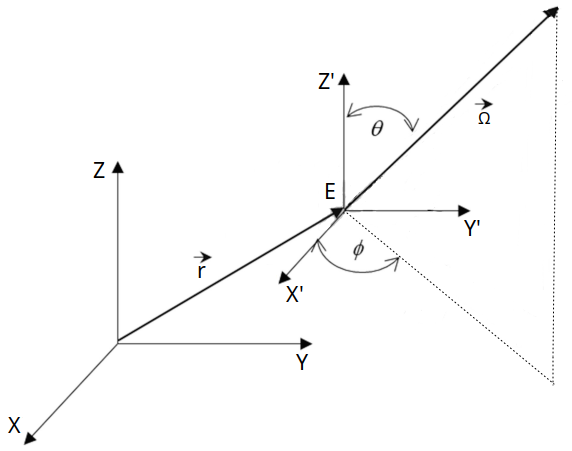
\includegraphics[width=0.5\textwidth]{figs/terna.png}
    \caption{Representación del espacio de fases con las variables $(E, x, y, z, \theta, \phi)$, donde $E$ es la energía, $x$, $y$ y $z$ son coordenadas espaciales y $\theta$ y $\phi$ son las variables direccionales.}
    \label{fig:terna}
\end{figure}

\section{Procesamiento del archivo de partículas original}
\subsection{Preprocesamiento del archivo de partículas}
Inicialmente, las partículas provenientes de la simulación Monte Carlo original se filtran seleccionando únicamente aquellas que se propagan hacia la región de interés y se separan las variables relevantes mencionadas, además del peso estadístico (\textit{weight}). Esta selección se realiza porque, en la siguiente etapa de simulación, la geometría ya no incluye la región anterior a la superficie de registro —es decir, la zona desde donde provienen originalmente las partículas—, y se asume un vacío en su lugar. Por lo tanto, sólo tiene sentido conservar aquellas partículas que se propagan hacia la región de interés. Las partículas que se dirigen en sentido opuesto no son relevantes para la simulación posterior, ya que en caso de que alguna partícula fuese a regresar por retrodispersión, dicho comportamiento ya está estadísticamente incorporado en la lista original de partículas, producto de la simulación completa previa. En la Tabla \ref{tab:estructura_trackfile} se presenta un ejemplo de la estructura típica de un archivo de partículas.

\begin{table}[h]
    \centering
    \begin{tabular}{ccccccc}
        \toprule
        \textbf{Partícula Nº} & \textbf{Letargía} & \textbf{x [cm]} & \textbf{y [cm]} & \textbf{$\mu$} & \textbf{$\phi$ [rad]} & \textbf{Peso estadístico} \\ 
        \midrule
        1       & 4.15 &  0.23  & -1.10 &  0.85 & 3.14 & 1.00 \\
        2       & 4.95 & -0.75  &  0.40 & 0.65 & 1.57 & 0.57 \\
        3       & 5.05 &  1.10  &  0.70 &  0.45 & 0.78 & 1.00 \\
        4       & 5.30 & -0.50  & -0.90 &  0.60 & 2.35 & 0.33 \\
        5       & 4.85 &  0.85  & -0.20 & 0.95 & 1.25 & 1.00 \\
        $\vdots$ & $\vdots$ & $\vdots$ & $\vdots$ & $\vdots$ & $\vdots$ & $\vdots$ \\[0.2cm]
        100000  & 5.00 &  0.10  &  0.55 & 0.70 & 0.95 & 0.99 \\
        \bottomrule
    \end{tabular}
    \caption{Ejemplo ilustrativo de la estructura típica de un archivo de partículas. El archivo original suele contener cientos de miles de partículas.}
    \label{tab:estructura_trackfile}
\end{table}

\subsection{Utilización de histogramas macro y micro}
La metodología desarrollada en este trabajo para aproximar distribuciones y correlaciones multidimensionales en el espacio de fases de partículas provenientes de simulaciones Monte Carlo se basa en un esquema combinado de histogramas macro y micro. Esta aproximación permite gestionar eficientemente grandes volúmenes de datos manteniendo una representación precisa de la información esencial del conjunto original de partículas.

Los histogramas macro son subdivisiones jerárquicas del espacio de fases, realizadas siguiendo un orden determinado por quien utiliza la herramienta. Por ejemplo, un posible orden es la letargía, seguida por las coordenadas espaciales (\textit{X}, \textit{Y}), y posteriormente por la dirección (\textit{$\mu$}, \textit{$\phi$}). Este procedimiento inicia dividiendo el conjunto original de partículas en macrogrupos según la primera variable elegida (por ejemplo, letargía). Cada macrogrupo así generado es posteriormente subdividido en nuevos macrogrupos en función de la siguiente variable (por ejemplo, la coordenada \textit{X}), repitiéndose este proceso de manera iterativa para cada variable subsiguiente. El resultado es una estructura jerárquica en forma de árbol, donde cada rama representa un subconjunto específico del archivo original de partículas, ya que incluye las cinco variables consideradas. Cada nodo en la rama corresponde a  una variable dentro de dicho subconjunto. En la Figura \ref{fig:estructura_jerarquica} se ilustra este procedimiento de subdivisión jerárquica del espacio de fases. Este método implementado presenta diferencias respecto al esquema empleado en trabajos anteriores \cite{Fairhurst2017Hist}, donde los macrogrupos y microgrupos eran construidos de forma cíclica, es decir, la discretización de cada variable consideraba simultáneamente la influencia de las demás. En contraste, en la implementación aquí desarrollada, los macrogrupos y microgrupos de la primera variable seleccionada se construyen sin referencia a las restantes, y a partir de esta primera discretización se procede con la segmentación de la siguiente variable, considerando únicamente las divisiones ya establecidas. De este modo, el orden en que se procesan las variables define una jerarquía en la cual cada nivel se construye condicionado por las particiones realizadas en los niveles anteriores, y no en función de variables aún no discretizadas.

\begin{figure}[h]
    \centering
    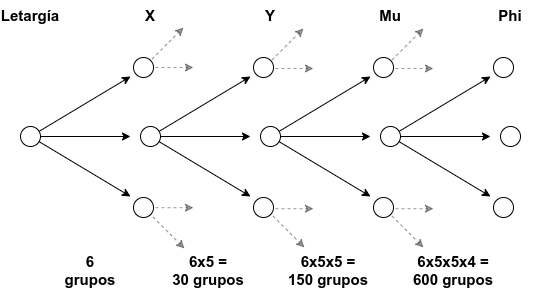
\includegraphics[width=0.8\textwidth]{grupos.png}
    \caption{Esquema ilustrativo de la estructura jerárquica de macrogrupos y microgrupos formando un árbol. Se resalta la jerarquía entre variables.}
    \label{fig:estructura_jerarquica}
\end{figure}

Este esquema tiene como objetivo capturar las correlaciones entre las variables del espacio de fases. Cada nodo o macrogrupo resultante comparte similitudes en todas las variables consideradas hasta ese nivel jerárquico. Por ejemplo, un macrogrupo particular tendrá partículas con distribuciones similares en letargía, coordenadas espaciales (\textit{X}, \textit{Y}), y dirección \textit{($\mu$)}, lo cual garantiza que la distribución restante en la última variable \textit{($\phi$)} refleje adecuadamente las correlaciones subyacentes en los datos.

Cabe destacar que, en la etapa de macrodiscretización, se utilizan histogramas con baja resolución debido al crecimiento exponencial en la cantidad total de grupos generados, dado que el número total de macrogrupos es producto del número de divisiones en cada variable. Un número excesivamente alto de divisiones podría conducir a subconjuntos con muy pocas partículas, comprometiendo la calidad estadística.

Una vez establecidos los macrogrupos, cada nodo es discretizado con histogramas micro, los cuales poseen una mayor resolución para representar detalladamente la distribución de cada variable dentro del subconjunto. Esta discretización se realiza ponderando por el peso estadístico, lo que permite conservar la importancia relativa de cada evento. A partir de los histogramas micro así construidos, se calcula la función de frecuencia acumulada, la cual es posteriormente normalizada para definir una distribución de probabilidad que pueda ser utilizada en el proceso de remuestreo. Sin embargo, es crucial controlar esta resolución para evitar reproducir el ruido estadístico presente en los datos originales, especialmente cuando se cuenta con un número reducido de partículas en el subconjunto.

La combinación de histogramas macro y micro permite obtener una aproximación eficiente y precisa de la distribución multidimensional del conjunto original, conservando las correlaciones entre las variables del espacio de fases. Esta estructura de histogramas multidimensionales representa, en síntesis, la información esencial extraída del archivo original de partículas para ser utilizada en simulaciones posteriores.

\subsection{Métodos de discretización aplicados a histogramas macro y micro}
En este trabajo se desarrollaron dos métodos de discretización (\textit{bineado}) aplicables tanto a los histogramas macro como a los micro. El primero es el \textit{bineado} uniforme, que consiste en dividir la distribución de la variable en estudio utilizando bines equiespaciados. Este método tiene la ventaja de ser sencillo y rápido en su implementación, pero presenta la desventaja de no poder capturar adecuadamente cambios abruptos o picos aislados en las distribuciones.

El segundo método, denominado \textit{bineado} adaptativo, consiste en realizar inicialmente un \textit{bineado} uniforme con una cantidad moderada de bines especificada por quien utiliza la herramienta. Luego, este \textit{bineado} inicial se refina iterativamente agregando nuevos bines donde la distribución estimada difiere en mayor medida respecto a la distribución original. El criterio para añadir un nuevo bin se basa en la comparación de la función de distribución acumulada (FDC) del \textit{bineado} actual con la FDC de la distribución original calculada con alta resolución. En cada iteración, se identifica el punto con la mayor diferencia absoluta entre ambas FDC, donde se coloca un borde de bin adicional. En el \textbf{Apéndice \ref{app:A}} se presenta un ejemplo de la implementación de este método.

Este enfoque adaptativo permite asignar mayor resolución donde existe una mayor cantidad de peso estadístico, y menor resolución donde el peso es escaso, logrando así un mejor seguimiento de las zonas críticas y un adecuado suavizado en regiones con poca estadística.

Además, debido a que la cantidad de partículas generalmente disminuye al profundizar en las ramas del árbol jerárquico, puede ser necesario utilizar una resolución decreciente en las discretizaciones, tanto para los histogramas macro como para los micro, lo cual también ha sido implementado en este trabajo.

Finalmente, en aquellos casos en que quien utiliza el código conozca previamente la existencia de cambios abruptos o picos específicos en la distribución, es posible informar manualmente al método sobre la ubicación de estos fenómenos, estableciendo bordes de bin específicamente en esos puntos para mejorar la precisión de la discretización.

\section{Remuestreo de partículas en simulaciones Monte Carlo subsecuentes}
El proceso de generación de partículas a partir de la información guardada en los histogramas multidimensionales implica:
\begin{enumerate}
    \item Generar un número pseudoaleatorio entre 0 y 1.
    \item Interpolar dicho número en la distribución acumulada normalizada de la variable raíz del árbol.
    \item Avanzar secuencialmente por las ramas del árbol determinando valores de las variables subsecuentes hasta obtener un conjunto completo de variables del espacio de fases.
\end{enumerate}

En la Figura \ref{fig:esquema_generacion_particulas} se ejemplifica el proceso de generación de partículas descrito previamente. En el caso particular de trabajar con cinco variables, se repetirá la generación de números pseudoaleatorios cinco veces consecutivas, obteniéndose así los cinco valores correspondientes de las variables. Cabe destacar que durante el remuestreo de la quinta variable no se generará un macrogrupo adicional, dado que esta es la última variable a muestrear y no existen más niveles en el árbol.

\begin{figure}[H]
    \centering
    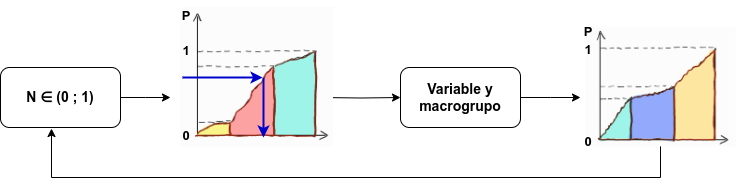
\includegraphics[width=\textwidth]{esquema5.png}
    \caption{Esquema ilustrativo del proceso secuencial de generación de partículas a partir de la distribución jerárquica guardada, resaltando el muestreo sucesivo mediante números pseudoaleatorios.}
    \label{fig:esquema_generacion_particulas}
\end{figure}

A través de este proceso es posible remuestrear nuevas partículas para la siguiente etapa de la simulación. Existen dos formas de integrar esta funcionalidad con \texttt{OpenMC}:

\begin{itemize}
    \item Una opción consiste en realizar, de forma \emph{offline}, el muestreo de una cantidad predeterminada de partículas y guardar sus propiedades en un archivo de partículas. Este archivo puede ser luego utilizado por \texttt{OpenMC} mediante su opción de simulación desde el modo de fuente \texttt{FileSource} implementado en el programa.
    
    \item Alternativamente, se puede ejecutar \texttt{OpenMC} con una fuente \texttt{HistogramSource}, definida \textit{ad hoc} y configurada mediante un archivo \texttt{XML}. En este caso, \texttt{OpenMC} accede directamente al árbol de histogramas durante la simulación y genera cada partícula \emph{on-the-fly}, lo que reduce significativamente el uso de memoria y evita la necesidad de almacenar archivos de partículas intermedios voluminosos.
\end{itemize}

Esta última funcionalidad fue incorporada en el contexto del presente trabajo, mediante la definición de una nueva clase de fuente en el código fuente de \texttt{OpenMC} en \texttt{C++} \cite{RepositorioKDSource2025} \cite{RepositorioOpenMCSource2025}. Se desarrollaron las estructuras necesarias en \texttt{C} para efectuar el muestreo desde histogramas multidimensionales, y se integraron con la \texttt{API} de \texttt{OpenMC} en \texttt{Python}, permitiendo así que los histogramas puedan ser cargados y utilizados dentro del flujo habitual de simulación. El objetivo principal de esta implementación es facilitar el uso práctico de la herramienta.


\section{Implementación computacional}

La implementación computacional de la metodología descrita en este capítulo se encuentra desarrollada y documentada en el \textbf{Apéndice \ref{app:B}}. En particular, se presentan los códigos elaborados en \texttt{Python}, \texttt{C} y \texttt{C++} que posibilitan la generación y manejo de los histogramas multidimensionales generados a partir del archivo original de partículas. Dichos histogramas se configuran mediante parámetros específicos definidos por quien utiliza la herramienta, tales como número y tipo de bines, así como el orden en que se procesan las variables del espacio de fases.

Asimismo, se documenta en detalle la integración realizada con \texttt{OpenMC}, incluyendo las modificaciones llevadas a cabo en su \textit{API} de \texttt{Python} y en su código fuente en \texttt{C++}, para permitir la generación \textit{on-the-fly} de partículas durante las simulaciones Monte Carlo subsecuentes.
